\chapter{Pendahuluan}
\label{chap:intro}
   
\section{Latar Belakang}
\label{sec:label}

Dengan adanya situasi pandemi Covid-19 mulai tahun 2020, seluruh kegiatan kuliah wajib dilaksanakan secara \textit{online}. Sebelum pandemi, kegiatan praktikum dan ujian kuliah pemrograman Teknik Informatika Unpar dilaksanakan di lab komputer, sehingga dapat di diawasi secara langsung oleh dosen dan asisten dosen .  Namun, pengawasan menjadi lebih sulit untuk dilakukan saat kuliah dilaksanakan secara \textit{online}. 

Pada mata kuliah pemrograman Teknik Informatika Unpar, dimanfaatkan SharIF Judge, sebuah \textit{online judge} untuk bahasa pemrograman C, C++, Java dan Python untuk mempermudah proses pengumpulan dan penilaian kode program. \textit{Online judge} adalah sebuah sistem \textit{online} yang berfungsi untuk mengevaluasi kode program yang dikumpulkan oleh pengguna. Kode program yang dikumpulkan akan dikompilasi dan diuji pada lingkungan yang serupa, kemudian diberi nilai berdasarkan hasil yang didapatkan \cite{judge}.

SharIF Judge (dengan IF kapital) adalah modifikasi cabang oleh Stillmen Vallian terhadap Sharif Judge (dengan if kecil) yang diciptakan oleh Mohammad Javad Naderi dengan \textit{framework} CodeIgniter dan Bash \cite{sharif}. Modifikasi ini dilakukan untuk menyesesuaikan Sharif Judge terhadap kebutuhan spesifik Teknik Informatika Unpar \cite{stillmen:sharif}.

Pada SharIF judge, pengumpulan kode dilakukan dengan mengunggah kode program, yang biasanya dibuat oleh mahasiswa dengan menggunakan aplikasi eksternal. Karena proses pembuatan kode program tidak terintegrasi, SharIF Judge tidak memiliki kemampuan untuk mengawasi proses pembuatan kode program. Sebelum pandemi, pengawasan dapat dilakukan secara langsung oleh dosen dan asisten dosen di lab komputer. Namun, ketika kuliah dilakukan secara \textit{online}, diperlukan cara lain untuk mengawasi mahasiswa. 

Pada skripsi ini, diimplementasikan {\it Integrated Development Environment} (IDE), sebuah aplikasi dengan kemampuan untuk mengedit, mengompilasi, dan menjalankan kode program pada SharIF Judge, sehingga seluruh proses pembuatan kode program dapat dilakukan langsung di dalam SharIF Judge. Dengan demikian, proses pembuatan kode terintegrasi pada SharIF Judge, dan dapat dimanfaatkan untuk pengawasan.

Gambar \ref{fig:1:step} menggambarkan tahapan penelitian SharIF Judge. Pada skripsi ini, diimplementasikan IDE pada SharIF Judge, sehingga seluruh proses pembuatan kode program dapat dilakukan langsung di dalam SharIF Judge. Pada penelitian selanjutnya, dapat ditambahkan fitur pada IDE untuk membantu pengawasan terhadap mahasiswa selama kegiatan kuliah, misalnya dengan menangkap dan memutar ulang ketikan pada IDE.

% \textit{Online judge} adalah sebuah sistem \textit{online} yang berfungsi untuk mengevaluasi kode program yang dikumpulkan oleh pengguna. Kode program kemudian dikompilasi dan diuji pada lingkungan yang serupa. \textit{Online judge} sering kali digunakan dalam sistem pemrograman kompetitif dan edukasi pemrograman \cite{judge}.

% Sharif Judge (dengan if kecil) adalah sebuah \textit{online judge} untuk bahasa pemrograman C, C++, Java dan Python. Perangkat lunak ini diciptakan oleh Mohammad Javad Naderi dan bersifat \textit{open
% source}. Sharif Judge dibangun dengan menggunakan \textit{framework} CodeIgniter dan Bash \cite{sharif}.

% SharIF Judge (dengan IF kapital) adalah modifikasi cabang dari Sharif Judge oleh Stillmen Vallian yang disesuaikan untuk kebutuhan spesifik Teknik Informatika Unpar. SharIF Judge digunakan pada beberapa mata kuliah pemrograman untuk mempermudah proses pengumpulan dan penilaian kode program \cite{stillmen:sharif}.

% Dengan adanya situasi pandemi Covid-19 mulai tahun 2020, seluruh kegiatan kuliah wajib dilaksanakan secara \textit{online}. Pada umumnya, kegiatan praktikum dan ujian pada mata kuliah pemrograman Teknik Informatika Unpar dapat diawasi secara langsung oleh dosen dan asisten dosen di lab komputer.  Namun, pengawasan menjadi lebih sulit untuk dilakukan saat kuliah dilaksanakan secara \textit{online}. Diperlukan sebuah cara untuk mengawasi mahasiswa selama kuliah \textit{online} berlangsung. 

% {\it Integrated Development Environment} (IDE) adalah sebuah aplikasi dengan fitur yang lengkap untuk membantu penggunanya dalam proses pengembangan kode. Sebuah IDE pada umumnya memiliki kemampuan untuk mengedit, mengompilasi, menjalankan, dan menguji kode program \cite{ide}.  Mahasiswa pada umumnya menggunakan aplikasi IDE seperti Netbeans untuk membuat kode program yang kemudian diunggah ke SharIF Judge untuk dinilai.

% Gambar \ref{fig:1:step} menggambarkan tahapan penelitian SharIF Judge. Pada skripsi ini, akan dibangun IDE pada SharIF Judge, sehingga seluruh proses pembangunan kode dapat dilakukan langsung di dalam SharIF Judge. Pada penelitian selanjutnya, dapat ditambahkan fitur pada IDE untuk membantu pengawasan terhadap mahasiswa selama kegiatan kuliah, misalnya dengan menangkap dan memutar ulang ketikan pada IDE.

\begin{figure}[H]
	\centering  
	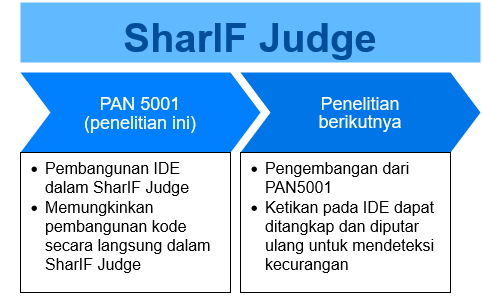
\includegraphics[scale=0.6]{Diagram/step.png}  
	\caption{Tahapan penelitian SharIF Judge}
	\label{fig:1:step} 
\end{figure} 

\section{Rumusan Masalah}
\label{sec:rumusan}
Rumusan masalah yang akan dibahas pada skripsi ini adalah sebagai berikut:
\begin{enumerate}
	\item Bagaimana mengimplementasikan {\it Integrated Development Environment} sehingga mahasiswa dapat mengedit, mengompilasi, dan menjalankan kode dalam SharIF Judge?
	\item Bagaimana tanggapan pengguna terhadap implementasi {\it Integrated Development Environment} pada SharIF Judge? 
\end{enumerate}


\section{Tujuan}
\label{sec:tujuan}
Tujuan yang ingin dicapai skripsi ini adalah sebagai berikut:
\begin{enumerate}
	\item Mengimplementasikan {\it Integrated Development Environment} sehingga mahasiswa dapat mengedit, mengompilasi, dan menjalankan kode dalam SharIF Judge.
	\item Mendapatkan umpan balik dari tanggapan pengguna terhadap implementasi {\it Integrated Development Environment} pada SharIF Judge.
\end{enumerate}

\section{Batasan Masalah}
\label{sec:batasan}
Pada pengerjaan skripsi ini terdapat batasan sebagai berikut:
\begin{itemize}
    \item Perangkat lunak SharIF Judge hanya digunakan pada lingkungan Teknik Informatika Unpar.
    \item Perangkat lunak hanya dapat diuji pada mata kuliah pemrograman di mana dosen pembimbing terlibat.
    \item Pada mata kuliah pemrograman, digunakan 2 \textit{judge} terpisah untuk latihan dan kuis. Berdasarkan keputusan dosen koordinator, perangkat lunak hanya akan diuji pada \textit{judge} latihan.
\end{itemize}


\section{Metodologi}
\label{sec:metlit}
Metodologi pengerjaan skripsi ini adalah sebagai berikut:
\begin{enumerate}
	\item Melakukan studi mengenai komponen yang diperlukan untuk membuat IDE berbasis web.
	\item Mempelajari struktur SharIF Judge.
	\item Merancang IDE berbasis web untuk SharIF Judge.
	\item Mengimplementasikan IDE berbasis web pada SharIF Judge.
	\item Melakukan pengujian dan eksperimen.
	\item Menulis dokumen skripsi.
\end{enumerate}

\section{Sistematika Pembahasan}
\label{sec:sispem}
Sistematika pembahasan skripsi ini adalah sebagai berikut:
\begin{itemize}
	\item Bab 1 Pendahuluan \\ Membahas latar belakang, rumusan masalah, tujuan, batasan masalah, metodologi, dan sistematika pembahasan.
	\item Bab 2 Landasan Teori \\ Membahas teori-teori yang berhubungan dengan penelitian ini, yaitu SharIF Judge, CodeIgniter 3, Twig, Bash, Integrated Development Environment, PDF.js, dan Ace.
	\item Bab 3 Analisis \\ Membahas analisis terhadap perangkat lunak SharIF Judge.
	\item Bab 4 Perancangan \\ Membahas perancangan fitur yang diimplementasikan pada SharIF Judge.
	\item Bab 5 Implementasi dan Pengujian \\ Membahas implementasi fitur pada SharIF Judge dan pengujian yang dilakukan.
	\item Bab 6 Kesimpulan dan Saran \\ Membahas kesimpulan dari penelitian ini dan saran untuk penelitian berikutnya.
\end{itemize}
